% \documentclass[aspectratio=169,14pt]{beamer}
\documentclass[xcolor=x11names]{beamer}
\maxdeadcycles=20
\usepackage[utf8]{inputenc}
\usepackage[english]{babel}
% \usepackage[brazil]{babel}
\usepackage[T1]{fontenc}
\usepackage{graphicx}
\usepackage{pax}
\usepackage{tikzscale}
\usepackage{appendix}
\usepackage{pgfplots}
\pgfplotsset{compat=newest}
\usepgfplotslibrary{groupplots}
\usepgfplotslibrary{dateplot}
\usepackage{xargs}
\usepackage{rotating}
\usepackage{pdflscape}
\usepackage{afterpage}
\usepackage[paper=A4,pagesize]{typearea}
\graphicspath{{../../figures/}} 
\usepackage{subcaption} 
\usepackage{hyperref}
\usepackage{amsmath,amssymb} 
\usepackage{indentfirst}
\usepackage[algo2e,linesnumbered,ruled]{algorithm2e}
\usepackage{algorithmic}
%%If desirable, the user can enable Times New Roman Fonts by uncommenting the next line. G.L.
% \usepackage{mathptmx}
\usepackage{pdfpages}
\usepackage{multirow}
\usepackage{color}
\usepackage{blindtext}
\usepackage{float}
\usepackage{nameref}
\usepackage{cleveref}
\usepackage{multicol}
\usepackage{listings}
\usepackage{enumerate}
\usepackage[acronym,toc]{glossaries}\makeglossaries
\usepackage{tikz}
\usepackage{ladder} %https://github.com/AurelienC/tex-ladder/blob/master/ladder.sty
\usetikzlibrary{arrows,shapes,automata,petri,external,arrows.meta}
	\tikzset{
	place/.style={
	circle,
	thick,
	draw=black!100, % draw=blue!75,
    % fill=blue!20,
    minimum size=6mm
  },
  extPlace/.style={
    circle,
    dotted,
    draw=black!100, % draw=blue!75,
    % fill=blue!20,
    minimum size=6mm
  },
  extTransition/.style={
    rectangle,
    dotted,
    fill=white,
    minimum width=8mm,
    inner ysep=0.7pt
  },
  transition/.style={
    rectangle,
    thick,
    fill=black,
    minimum width=8mm,
    inner ysep=0.7pt
  },
  extTimedtransition/.style={
    rectangle,
    dotted,
    fill=white,
    minimum width=8mm,
    inner ysep=2pt
  },
  timedtransition/.style={
    rectangle,
    thick,
    fill=white,
    minimum width=8mm,
    inner ysep=2pt
  },
  inhibitor/.style={-o},
  text/.style={}
}

\makeatletter
\tikz@def@grow@tokens{2}{1}{-1.5}{0}
\tikz@def@grow@tokens{2}{2}{1.5}{0}
% \tikz@def@grow@tokens{3}{1}{-1}{0}
% \tikz@def@grow@tokens{3}{2}{0}{1}
% \tikz@def@grow@tokens{3}{3}{1.5}{-1}
\makeatother


\definecolor{darkblue}{rgb}{0,0,0.3}
\definecolor{blue}{rgb}{0,0,0.5}
\definecolor{color1}{rgb}{1,0.2,0.3}
\definecolor{color2}{rgb}{0.05490196078,0.41176470588,0.13333333333}
% rgb(14, 105, 34)

\definecolor{color3}{rgb}{0.2,0.2,0.8}
% hyperref setup
\hypersetup{
  % pdftitle={\title},
  pdfauthor={Rafael Accácio Nogueira},
  pdfcreator={Rafael Accácio Nogueira},     
  bookmarksopen=true,         
  bookmarksopenlevel=1,       
  colorlinks=true, % false => boxes 
  linkcolor=blue,
  filecolor=red,  
  urlcolor=blue,  
  citecolor=blue,              
  pdfstartview=Fit,          
  pdfpagemode=UseOutlines,    % this is the option you were lookin for
  pdfpagelayout=TwoPageRight,
}

\makeatletter
\let\stdchapter\chapter
\renewcommand*\chapter{%
  \@ifstar{\starchapter}{\@dblarg\nostarchapter}}
\newcommand*\starchapter[1]{\stdchapter*{#1}}
\def\nostarchapter[#1]#2{
  \stdchapter[#1]{\protect\hyperlink{tocsection}{#1}}}
\makeatother

\makeatletter
\let\stdsection\section
\renewcommand*\section{%
  \@ifstar{\starsection}{\@dblarg\nostarsection}}
\newcommand*\starsection[1]{\stdsection*{#1}}
\def\nostarsection[#1]#2{
  \stdsection[#1]{\protect\hyperlink{tocsection}{#1}}}
\makeatother

\makeatletter
\let\stdsubsection\subsection
\renewcommand*\subsection{%
  \@ifstar{\starsubsection}{\@dblarg\nostarsubsection}}
\newcommand*\starsubsection[1]{\stdsubsection*{#1}}
\def\nostarsubsection[#1]#2{
  \stdsubsection[#1]{\protect\hyperlink{tocsection}{#1}}}
\makeatother

\makeatletter
\let\stdsubsubsection\subsubsection
\renewcommand*\subsubsection{%
  \@ifstar{\starsubsubsection}{\@dblarg\nostarsubsubsection}}
\newcommand*\starsubsubsection[1]{\stdsubsubsection*{#1}}
\def\nostarsubsubsection[#1]#2{
  \stdsubsubsection[#1]{\protect\hyperlink{tocsection}{#1}}}
\makeatother

\let\oldtoc\tableofcontents
\renewcommand{\tableofcontents}{\pagebreak\hypertarget{tocsection}{}\label{tocsection}\oldtoc}


\newcommand{\figplaceholder}[2]{
	\begin{figure}[H]
		\begin{center}	
			\rule{8cm}{8cm}
			\caption{\todo[FORGOT TO INCLUDE FIGURE]{#1 (placeholder)}}
			\label{fig:#2}
		\end{center}
	\end{figure}
}

\newif\ifdebug
\newcommand{\draft}{\debugtrue}
\newcommand{\final}{\debugfalse}
\newcommand{\todo}[2][FORGOT TO DO SOMETHING]{\ifdebug {\color{red}#2}\else \PackageError{}{#1}{}\fi}
\newcommand\doing[1]{\ifdebug {\color{blue}#1}\else \PackageError{}{FORGOT TO DO SOMETHING}{}\fi}
\newcommand\warning[1]{\ifdebug {\color{red}#1}\fi}
\newcommand\note[1]{\ifdebug {\color{orange}#1}\fi}

\usepackage{fancyhdr}
\pagestyle{fancy}

\fancyhead[L]{\warning{DRAFT}}
\fancyhead[R]{\warning{DEBUG ON}}

\fancyfoot[L]{\warning{TURN DEBUG OFF}}
\fancyfoot[R]{\warning{DRAFT}}

\newtheorem{theorem}{Theorem}
\numberwithin{theorem}{chapter}

\newtheorem{example}{Example}
\numberwithin{example}{chapter}

\newtheorem{definition}{Definition}
\numberwithin{definition}{chapter}

\newtheorem{observation}{Remark}
\numberwithin{observation}{chapter}

\usepackage[export]{adjustbox}

\newcommand{\includetikzfigure}[2][]{
    \ifdebug {\includegraphics[#1]{#2.pdf}}
    \else  \includegraphics[#1]{#2}\fi
}

\newcommand{\addtikzfigureLandscape}[4][width=0.8\textwidth]{
\KOMAoptions{paper=landscape}
\recalctypearea
  \vspace*{\fill}
  \begin{figure}[H]
    \centering
    \ifdebug {\includegraphics[#1]{#2.pdf}}
    \else  \includegraphics[#1]{#2}\fi
    \caption{#3}
    \label{fig:#4}
  \end{figure}
  \vspace*{\fill}
\KOMAoptions{paper=portrait}
\recalctypearea
}

\newcommand{\addtikzfigureLandscapeAthree}[4][width=0.8\textwidth]{
\KOMAoptions{paper=a3,paper=landscape}
% \KOMAoptions{paper=landscape}
\recalctypearea
  \begin{figure}[H]
    \vspace{-2cm}
    \centering
    \ifdebug {\centerline{\includegraphics[#1]{#2.pdf}}}
    \else  \centerline{\includegraphics[#1]{#2}}
\fi
    % \caption{#3}
    % \label{fig:#4}
  \end{figure}
\KOMAoptions{paper=a4,paper=portrait}
\recalctypearea
}

% \newcommand{\addtikzfigureVertCent}[3]{
% \KOMAoptions{paper=landscape}
% \recalctypearea
% % \begin{landscape}
% \vspace*{\fill}
%   \begin{figure}[H]
%     % \centering
%     % \resizebox{\hsize}{!}{
%     % \input{#1}
%      \includegraphics[width=1.15\textwidth]{#1}
%     % }
%     \caption{#2}
%     \label{fig:#3}
%   \end{figure}
% \vspace*{\fill}
% % \end{landscape}
% \KOMAoptions{paper=portrait}
% \recalctypearea
% }

\newcolumntype{P}[1]{>{\centering\arraybackslash}p{#1}}
\newcolumntype{M}[1]{>{\centering\arraybackslash}m{#1}}
\definecolor{keywordstyle}{rgb}{0,0,0.82}
\definecolor{commentstyle}{rgb}{0,0.6,0}
\definecolor{numberstyle}{rgb}{0.5,0.5,0.5}
\definecolor{stringstyle}{rgb}{0.58,0,0.82}

% Listing options
\lstset{ 
  % backgroundcolor=\color{white},   % choose the background color; you must add \usepackage{color} or \usepackage{xcolor}; should come as last argument
  basicstyle=\footnotesize,        % the size of the fonts that are used for the code
  breakatwhitespace=false,         % sets if automatic breaks should only happen at whitespace
  breaklines=true,                 % sets automatic line breaking
  captionpos=t,                    % sets the caption-position to bottom
  commentstyle=\color{commentstyle},    % comment style
  deletekeywords={...},            % if you want to delete keywords from the given language
  escapeinside={\%*}{*)},          % if you want to add LaTeX within your code
  extendedchars=true,              % lets you use non-ASCII characters; for 8-bits encodings only, does not work with UTF-8
  % firstnumber=1000,                % start line enumeration with line 1000
  % frame=single,	                   % adds a frame around the code
  keepspaces=true,                 % keeps spaces in text, useful for keeping indentation of code (possibly needs columns=flexible)
  keywordstyle=\color{keywordstyle},       % keyword style
  % language=Octave,                 % the language of the code
  morekeywords={*,...},            % if you want to add more keywords to the set
  numbers=left,                    % where to put the line-numbers; possible values are (none, left, right)
  numbersep=10pt,                   % how far the line-numbers are from the code
  numberstyle=\tiny\color{numberstyle}, % the style that is used for the line-numbers
  rulecolor=\color{black},         % if not set, the frame-color may be changed on line-breaks within not-black text (e.g. comments (green here))
  showspaces=false,                % show spaces everywhere adding particular underscores; it overrides 'showstringspaces'
  showstringspaces=false,          % underline spaces within strings only
  showtabs=false,                  % show tabs within strings adding particular underscores
  stepnumber=2,                    % the step between two line-numbers. If it's 1, each line will be numbered
  stringstyle=\color{stringstyle},     % string literal style
  tabsize=2,	                   % sets default tabsize to 2 spaces
  title=\lstname                   % show the filename of files included with \lstinputlisting; also try caption instead of title
}

%% as seen in https://tex.stackexchange.com/a/183682/143332
\makeatletter
\newcommand\Autoref[1]{\@first@ref#1,@}
\def\@throw@dot#1.#2@{#1}% discard everything after the dot
\def\@set@refname#1{%    % set \@refname to autoefname+s using \getrefbykeydefault
    \edef\@tmp{\getrefbykeydefault{#1}{anchor}{}}%
    \xdef\@tmp{\expandafter\@throw@dot\@tmp.@}%
    \ltx@IfUndefined{\@tmp autorefnameplural}%
         {\def\@refname{\@nameuse{\@tmp autorefname}s}}%
         {\def\@refname{\@nameuse{\@tmp autorefnameplural}}}%
}
\def\@first@ref#1,#2{%
  \ifx#2@\autoref{#1}\let\@nextref\@gobble% only one ref, revert to normal \autoref
  \else%
    \@set@refname{#1}%  set \@refname to autoref name
    \@refname~\ref{#1}% add autoefname and first reference
    \let\@nextref\@next@ref% push processing to \@next@ref
  \fi%
  \@nextref#2%
}
\def\@next@ref#1,#2{%
   \ifx#2@ and~\ref{#1}\let\@nextref\@gobble% at end: print and+\ref and stop
   \else, \ref{#1}% print  ,+\ref and continue
   \fi%
   \@nextref#2%
 }
 \makeatother

\newcommand{\colvec}[2][1]{%
  \scalebox{#1}{%
    \renewcommand{\arraystretch}{.7}%
    $\begin{bmatrix}#2\end{bmatrix}$%
  }
}


%%% Local Variables:
%%% mode: latex
%%% TeX-master: "./monografia.tex"
%%% End:

\usetheme[pageofpages=/,% String used between the current page and the
% total page count.
bullet=circle,% Use circles instead of squares for bullets.
titleline=true,% Show a line below the frame title.
alternativetitlepage=true,% Use the fancy title page.
titlepagelogo=poli-logo.pdf,% Logo for the first page.
watermark=polilogo_transp,% Watermark used in every page.
watermarkheight=0px,% Height of the watermark.
watermarkheightmult=0,% The watermark image is 4 times bigger
% than watermarkheight.
]{Torino}
\usefonttheme[onlymath]{serif}
\usecolortheme{blue}

\usefonttheme{serif}

\definecolor{lettercolor}{rgb}{0, 0,  0}
\setbeamertemplate{blocks}[rounded][shadow=false]







%%% Local Variables:
%%% mode: latex
%%% TeX-master: "presentation"
%%% End:

% \useinnertheme{default}
\useoutertheme[subsection=true,shadow,footline=authorinstitutetitle]{miniframes}

\defbeamertemplate*{footline}{shadow theme}
{%
 \leavevmode%
 \hbox{\begin{beamercolorbox}[wd=.25\paperwidth,ht=2.5ex,dp=1.125ex,leftskip=.3cm plus1fil,rightskip=.3cm]{author in head/foot}%
   \usebeamerfont{author in head/foot}\insertframenumber\,/\,\inserttotalframenumber\hfill\insertshortauthor
 \end{beamercolorbox}%
 \begin{beamercolorbox}[wd=.75\paperwidth,ht=2.5ex,dp=1.125ex,leftskip=.3cm,rightskip=.3cm plus1fil]{title in head/foot}%
   \usebeamerfont{title in head/foot}\insertshorttitle%
 \end{beamercolorbox}}%
 \vskip0pt%
}

\definecolor{lettercolor}{rgb}{0, 0.2,  0.5}
\usefonttheme{serif}
\usepackage{palatino}
\setbeamerfont{title like}{shape=\scshape}
\setbeamerfont{frametitle}{shape=\scshape}
\setbeamercolor*{lower separation line head}{bg=DeepSkyBlue4}
%\setbeamercolor*{normal text}{fg=black,bg=white}
\setbeamercolor*{alerted text}{fg=red!100}
\setbeamercolor*{example text}{fg=black}
\setbeamercolor*{structure}{fg=lettercolor}%fg=lettercolor
\setbeamercolor*{normal text}{fg=lettercolor,bg=BgColor!10}
\setbeamercolor*{frametitle}{fg=lettercolor}
\setbeamercolor*{palette tertiary}{fg=black,bg=black!10}
\setbeamercolor*{palette quaternary}{fg=black,bg=black!10}
\setbeamercolor*{block title}{fg=lettercolor,bg=white}
\setbeamercolor*{block body}{fg=lettercolor,bg=white}
\setbeamertemplate{blocks}[rounded][shadow=true]
\addtobeamertemplate{block begin}{\pgfsetfillopacity{0.7}}{\pgfsetfillopacity{1}}%0.7 / 1
\addtobeamertemplate{block alerted begin}{\pgfsetfillopacity{0.5}}{\pgfsetfillopacity{1}}%0.5/1

\logo{\pgfputat{\pgfxy(-6,-0.24)}{\pgfbox[center,base]{\pgfsetfillopacity{0.09}{
\includegraphics[width=1.1\textwidth]{pres_fondo1.png}}}}}

\usepackage{appendixnumberbeamer}
\usepackage{natbib}
% \usepackage{biblatex}
\definecolor{BgColor}{rgb}{ 0.98823529,  0.98823529,  0.58039216}
\author{Rafael Accácio Nogueira}
\title{Identificação de um Sistema de Manufatura Didático}
\institute{Email: raccacio@poli.ufrj.br}
\date{19 de Julho de 2019}
\usepackage[absolute,overlay]{textpos} %needed for textblock
\usepackage[timeinterval=60]{tdclock}
% \setbeameroption{show notes on second screen}
\setbeamertemplate{note page}{\pagecolor{white}\vfill\insertnote\vfill}
\makeindex


\begin{document}
\begin{frame}[t,plain]
	\titlepage
\end{frame}
%%% Local Variables:
%%% mode: latex
%%% TeX-master: "apresentation"
%%% End:

% {
\usebackgroundtemplate{%

  \makebox[0pt][t]{
\includegraphics[width=1.185\hsize]{pres_title1.pdf}}}

\begin{frame}[plain]
\vspace*{8mm}
\title{Identificação de um Sistema de Manufatura Didático}
\author{\vspace{-.3cm} Rafael Accácio Nogueira}
\date{\vspace{1cm} 19 de julho de 2019}
\titlepage
\end{frame}
}


\setbeamertemplate{section in toc}[square]
\setbeamertemplate{subsection in toc}[square]
\newcommand{\eachsectiononlycurrentsubsections}{\AtBeginSection[]{
	\begin{frame}
	\frametitle{Sumário}
	%			\linespread{1.3}
	\tableofcontents[currentsection,sectionstyle=show/hide,subsectionstyle=show/show/hide]
\end{frame}
}}
\eachsectiononlycurrentsubsections

\begin{frame}{Sumário}\note{Falar o sumário}
% \begin{multicols}{2}
	\tableofcontents[subsectionstyle=hide/hide]
% \end{multicols}
\end{frame}
      
%%% Local Variables:
%%% mode: latex
%%% TeX-master: "presentation"
%%% End:


\chapter{Introduction}
In a world where the majority of the population lives in industrial societies,
and machines take part on the bulk of the production of almost all goods: from
food to cosmetics and drugs, from toothbrushes to automobiles, 
a well-paced throughput it is crucial, and any non expected halt on the
production or change can be disastrous, producing sometimes multimillionaire debts,
provoking a snowball effect, affecting the economy and consequentially the welfare of the society.

A diverse number of causes of the halt or change of the throughput can be
accounted for. Some are as simple as a power outage, or a component malfunction,
but nowadays there are other players. As the industry \textsl{walks}, or even
better \textsl{runs}, towards the so called Fourth Industrial Revolution, the industry
urges the use of \textit{connected sensors}, since the Internet of Things is the
fashion these days, but the concerns about cyber security are now and again neglected.   
So hackers can infiltrate the system, and depending of the infrastructure
halt or change somehow the production throughput.

Cyber security is not the theme of this thesis but its theme is another important concern to a
well-paced throughput, failure detection.

As great part of the manufacture facilities uses conveyor
belts, pneumatic cylinders and digital sensors, it is very common to see \PLCs



\PLC 




\acr{oi}{oi}{oi}
\oi





khe  the most simple as  In order to prevent these effects lots of 
\todo{ objetivo mostrar que o metodo pode funcionar 
com comportamento paraelo mostrar a escabilidade
}
\doing{the objective of this thesis is to show that the \DAOCT model works with
  systems that presents parallel behavior dividing themand can be used to scalability }
\section{Thesis Outline}
\label{sec:thesisOutline}






%%% Local Variables:
%%% mode: latex
%%% TeX-master: "../monografia.tex"
%%% End:

\section{Identificação}
\tikzstyle{every picture}+=[remember picture]

\begin{frame}{}
  \note{
    \begin{itemize}
    \item Caixa preta, não se conhece a planta
    \item Observar sinais de entrada e saida do controlador
    \item criar modelo a partir deles 
    \end{itemize}
  }

\only<1>{ 
\begin{figure}[H]
  \centering\small
     \begin{tikzpicture}
        % \draw[help lines,xstep=1,ystep=1] (0,0) grid (10,10);
        % \foreach \x in {0,1,...,10} { \node [anchor=north] at (\x,0) {\x}; }
        % \foreach \y in {0,1,...,10} { \node [anchor=east] at (0,\y) {\y}; }
        
        \draw[very thick,rounded corners] (3.5,0) rectangle (6.5,1.5);
        \draw[very thick,rounded corners] (0.5,2) rectangle (3.5,3.5);
        \draw[very thick,rounded corners] (6.5,2) rectangle (9.5,3.5);
        \draw[very thick,rounded corners] (3.5,4.5) rectangle (6.5,6);
        \draw (5,5.25) node {Controlador};
        \draw (5,0.75) node {Planta};
        \draw (2,2.75) node {Atuadores};
        \draw (8,2.75) node {Sensores};

        % actuators to plant
        \draw[->,>=stealth, thick] (2,2) -- (2,0.75) -- (3.5,0.75);

        % controller to actuators
        \draw[->,>=stealth, thick] (3.5,5.25) -- (2,5.25) -- (2,3.5);

        % Plant to sensors
        \draw[->,>=stealth, thick] (6.5,0.75) -- (8,0.75) -- (8,2);

        % Sensors to controller
        \draw[->,>=stealth, thick] (8,3.5) -- (8,5.25) -- (6.5,5.25);

        % \draw[->,>=stealth, thick] (2,4) -- (10,4);
        % \draw[fill] (2,4) circle(.05);

        % \draw[->,>=stealth, thick] (8,4.5) -- (10,4.5);
        % \draw[fill] (8,4.5) circle(.05);

        % \draw (11.4,4.5) node {Sinais};
        % \draw (11.4,4.15) node {observados};

        % \draw (1.5,5.75) node {Saídas do Controlador};
        % \draw (8.5,5.75) node {Entradas do Controlador};

      \end{tikzpicture}
 % \begin{minipage}{1.2\wd0}
 %  \centering
 %   \usebox0
  \caption{Sinais Observados de um sistema em malha fechada.}
 % \end{minipage}
    \label{fig:obsSignals}
  \end{figure}}
\only<2>{ 
\begin{figure}[H]
  \centering\small
     \begin{tikzpicture}
        % \draw[help lines,xstep=1,ystep=1] (0,0) grid (10,10);
        % \foreach \x in {0,1,...,10} { \node [anchor=north] at (\x,0) {\x}; }
        % \foreach \y in {0,1,...,10} { \node [anchor=east] at (0,\y) {\y}; }
        
        \draw[very thick,rounded corners] (3.5,0) rectangle (6.5,1.5);
        \draw[very thick,rounded corners] (0.5,2) rectangle (3.5,3.5);
        \draw[very thick,rounded corners] (6.5,2) rectangle (9.5,3.5);
        \draw[very thick,rounded corners] (3.5,4.5) rectangle (6.5,6);
        \draw (5,5.25) node {Controlador};
        \draw (5,0.75) node {Planta};
        \draw (2,2.75) node {Atuadores};
        \draw (8,2.75) node {Sensores};

        % actuators to plant
        \draw[->,>=stealth, thick] (2,2) -- (2,0.75) -- (3.5,0.75);

        % controller to actuators
        \draw[->,>=stealth, thick] (3.5,5.25) -- (2,5.25) -- (2,3.5);

        % Plant to sensors
        \draw[->,>=stealth, thick] (6.5,0.75) -- (8,0.75) -- (8,2);

        % Sensors to controller
        \draw[->,>=stealth, thick] (8,3.5) -- (8,5.25) -- (6.5,5.25);

        \draw[->,>=stealth, thick] (2,4) -- (10,4);
        \draw[fill] (2,4) circle(.05);

        \draw[->,>=stealth, thick] (8,4.5) -- (10,4.5);
        \draw[fill] (8,4.5) circle(.05);

        \draw (11.4,4.5) node {Sinais};
        \draw (11.4,4.15) node {observados};

        % \draw (1.5,5.75) node {Saídas do Controlador};
        % \draw (8.5,5.75) node {Entradas do Controlador};

      \end{tikzpicture}
 % \begin{minipage}{1.2\wd0}
 %  \centering
 %   \usebox0
  \caption{Sinais Observados de um sistema em malha fechada.}
 % \end{minipage}
    \label{fig:obsSignals}
  \end{figure}}
\end{frame}

\begin{frame}
  Vetores de Entrada/Saída  \note{
    \begin{itemize}
    \item armazenar os vetores de entrada e usar para
      gerar a linguagem do modelo
  \item a linguagem produzida pelo modelo deve ser o mais similar possível a
    linguagem original do sistema 
  \end{itemize}
}
\begin{equation*}
\mathbf{u}(t_1)=
\begin{bmatrix}
  i_1(t_1)&
  \dots&
  i_{m_i}(t_1)&
  o_1(t_1)&
  \dots&
  o_{m_o}(t_1)
\end{bmatrix}^T
\end{equation*}
\end{frame}
\begin{frame}{Relação entre Linguagens}
  \note{
    \begin{itemize}
    \item Linguagem original do sistema, Linguagem observada e Linguagem
      identificada
    \item preta A parte do sistema original que não foi identificada, gera
      falsos alarmes já que o que foi considerado uma falha pode estar presente
      na linguagem original do sistema mas não ter sido identificado 
    \item vermelha corresponde a parte identificada que não está presente na
      linguagem original, gera falhas não detectadas
    \item objetivo é minimizar as duas áreas 
    \end{itemize}
  }
  \begin{figure}[H]
 \sbox0{
   \includegraphics[width=0.7\textwidth]{vennDiagramLanguagesPresentation.tikz}
 }
  % \centering
 \begin{minipage}{1.2\wd0}
  \centering
   \usebox0
   \caption{Relação entre $L_{Orig}$, $L_{OrigNI}$,
    $L_{Obs}$, $L_{Exc}$ e $L_{Iden}$}.
 \end{minipage}
  \label{fig:languagesVenn}
\end{figure}
\end{frame}

\begin{frame}{Redução de Linguagens}
\begin{itemize}
\item Problema: minimizar $L_{OrigNI}$ \pause \\$L_{Orig}$ não é conhecida \pause
\item \cite{klein2005fault}:  $\exists n_0\in\mathbb{N}$ no qual
  $L_{Orig}^{\leq n_0}\backslash L_{Obs}^{\leq n_0}\approx \emptyset $  \pause \\
Considerando que $L_{Obs}\subseteq L_{Iden}$ então  $L_{Iden}^{\leq n_0}\approx
\emptyset$  \pause
\item Suposição: Todas sequências de eventos com comprimento $n_0 + 1$ são observados  \pause
\item Modelo identificado deve reduzir $L_{Exc}$ \pause
  \item \cite{moreira2018enhanced} apresentam modelo \\Derministic Automaton with
    Outputs and Conditional Transitions (DAOCT) 
\end{itemize}

\note{
\begin{enumerate}
  \item
\item Se o sistema for observado tempo o suficiente existe um número $n_0$ para
    o qual o conjunto das sequências de eventos de comprimento menor que $n_0$
    das linguagem observada e original são aproximadamente iguais
\item Neste trabalho supomos que todos eventos
\item
\item Modelo que utiliza índice de caminhos para reduzir a linguagem excedente, comparando com outros modelos da literatura
\end{enumerate}
}
\end{frame}
\begin{frame}
\begin{definition}[DAOCT]
  \label{def:daoct}
  \small
  \[ DAOCT = (X,\Sigma,f,\lambda,R,\theta, x_0,X_f)\]
  \indent X conjunto de \textbf{estados} \\
  \indent $\Sigma$ conjunto de \textbf{eventos}\\
  \indent $\Omega \subset \mathbb{N}_1^{m_i+m_o} $ conjunto de \textbf{vetores E/S}\\
  \indent $f:  X \times \Sigma^\star \rightarrow X$ função de  \textbf{transição determinística}\\
  \indent $\lambda : X \rightarrow \Omega$ função de  \textbf{saídas do stado}\\
  \indent $R = {1,2,\dots,r}$ conjunto de \textbf{indices dos caminhos}\\
  \indent $\theta : X \times \Sigma \rightarrow 2^R$ função de \textbf{estimação
    de caminho}\\
  \indent $x_0$ \textbf{estado inicial} \\
  \indent $X_f \subseteq X $ conjunto de \textbf{estados finais}
\end{definition}
\note{
\begin{enumerate}
\item usa sequências de vetores de entrada e saídas e eventos, denominados caminhos  
\end{enumerate}
}
\end{frame}


\begin{frame}{Caminhos Observados}
  \note{
\begin{itemize}
\item Os caminhos são formados por vetores e eventos
\item Os eventos caracterizam a mudança do vetor E\slash S, exemplo a bordo de
  subida de 1 ...
\end{itemize}}
  \setlength\arraycolsep{2pt}  \vspace{-0.5cm}
\small \begin{align*}
  p_1&= \left(\colvec{1\\0\\0},a,\colvec{1\\1\\0},b,\colvec{0\\1\\1},c,\colvec{0\\0\\0},d,\colvec{0\\0\\1},e,\colvec{1\\0\\0}\right) \\
  p_2&= \left(\colvec{1\\0\\0},g,\colvec{0\\0\\0},h,\colvec{1\\1\\0},b,\colvec{0\\1\\1},c,\colvec{0\\0\\0},i,\colvec{1\\0\\0},j,\colvec{0\\1\\1},l,\colvec{1\\0\\0}\right) \\
  p_3&= \left(\colvec{1\\0\\0},g,\colvec{0\\0\\0},h,\colvec{1\\1\\0},b,\colvec{0\\1\\1},i,\colvec{1\\1\\1},m,\colvec{0\\0\\0},d,\colvec{0\\0\\1},n,\colvec{1\\1\\0}\right) \\
       \end{align*}
\centering
      \only<2>{$a$ = $\uparrow$2, $b$ = $\downarrow$1$\uparrow$3, \dots} 
\end{frame}
\newcommand{\vu}{\mathbf{u}}

\begin{frame}{Caminhos Modificados}
  \note{Para diferenciar cada vetor é criada a variável livre k, que é usada
    para armazenar os $k-1$ vetores anteriores gerando caminhos modificados usando a seguinte fórmula }
\begin{equation}
  \label{eq:modifiedPath}
 p_i^k= (y_{i,1},\sigma_{i,1},y_{i,2},\sigma_{i,2},\dots,\sigma_{i,l_1-1},y_{i,l_i}) 
\end{equation}
onde 
\begin{equation}
  \label{eq:modifiedPathb}
y_{i,j}=\begin{cases}
    (\vu_{i,j-k+1},\dots,\vu_{i,j}),& \quad \text{if } k\leq j\leq l_i\\
    (\vu_{i,1},\dots,\vu_{i,j}),  & \quad \text{if } j<k
  \end{cases}
\end{equation}
\end{frame}


% http://www.texample.net/tikz/examples/beamer-arrows/
\begin{frame}{Caminhos Modificados}
  \note{
    Como que para $k=1$ são armazenados $0$ vetores anteriores, o
        modificado é igual o observado.
      } 
  \setlength\arraycolsep{2pt}
 $\bullet$ $k=2$
 \small
 \begin{align*}
   p_1&= \left(\tikz[baseline]{
            \node[anchor=base] (n1)
            {$\colvec{1\\0\\0}$};
        },a,\tikz[baseline]{
            \node[anchor=base] (n2)
            {$\colvec{1\\1\\0}$};
        },b,\tikz[baseline]{
            \node[anchor=base] (n3)
            {$\colvec{0\\1\\1}$};
        },c,\colvec{0\\0\\0},d,\colvec{0\\0\\1},e,\colvec{1\\0\\0}\right)
   \tikz[baseline] \node[coordinate] (baba) {};
\end{align*}
 \begin{align*}
  p_1^2&= \left(\tikz[baseline]{
            \node[anchor=base] (t1)
            {$\colvec{1\\0\\0}$};
        },a,\tikz[baseline]{
            \node[anchor=base] (t2)
            {$\colvec{1&1\\0&1\\0&0}$};
        },b,\tikz[baseline]{
            \node[anchor=base] (t3)
            {$\colvec{1&0\\1&1\\0&1}$};
        },c,\colvec{0&0\\1&0\\1&0},d,\colvec{0&0\\0&0\\0&1},e,\colvec{0&1\\0&0\\0&0}\right) \\ 
 \end{align*}
 \begin{tikzpicture}[overlay]
        \only<2>{\path[->,>=stealth,red] (n1) edge [bend left] (t1);}
        \only<3>{\path[->,>=stealth,red] (n1) edge [bend right] (t2);}
        \only<3>{\path[->,>=stealth,red] (n2) edge [bend left] (t2);}
        \only<4>{\path[->,>=stealth,red] (n2) edge [bend right] (t3);}
        \only<4>{\path[->,>=stealth,red] (n3) edge [bend left] (t3);}
      \end{tikzpicture}
\end{frame}


\begin{frame}{Caminhos Modificados}\note{14 vetores únicos enquanto no original com $k=1$
    só existem 6}
  \setlength\arraycolsep{2pt}
 $\bullet$ $k=2$
  \small \begin{align*}
  p_1^2&= \left(\colvec{1\\0\\0},a,\colvec{1&1\\0&1\\0&0},b,\colvec{1&0\\1&1\\0&1},c,\colvec{0&0\\1&0\\1&0},d,\colvec{0&0\\0&0\\0&1},e,\colvec{0&1\\0&0\\0&0}\right) \\ 
  p_2^2&= \left(\colvec{1\\0\\0},g,\colvec{1&0\\0&0\\0&0},h,\colvec{0&1\\0&1\\0&0},b,\colvec{1&0\\1&1\\0&1},c,\colvec{0&0\\1&0\\1&0},i,\colvec{0&1\\0&0\\0&0},j,\colvec{1&0\\0&1\\0&1},l,\colvec{0&1\\1&0\\1&0}\right) \\
  p_3^2&= \left(\colvec{1\\0\\0},g,\colvec{1&0\\0&0\\0&0},h,\colvec{0&1\\0&1\\0&0},b,\colvec{1&0\\1&1\\0&1},i,\colvec{0&1\\1&1\\1&1},m,\colvec{1&0\\1&0\\1&0},d,\colvec{0&0\\0&0\\0&1},n,\colvec{0&1\\0&1\\1&0}\right) \\
\end{align*}
\end{frame}



\begin{frame}{}
  \begin{figure}[H]
    \footnotesize
    \centering
    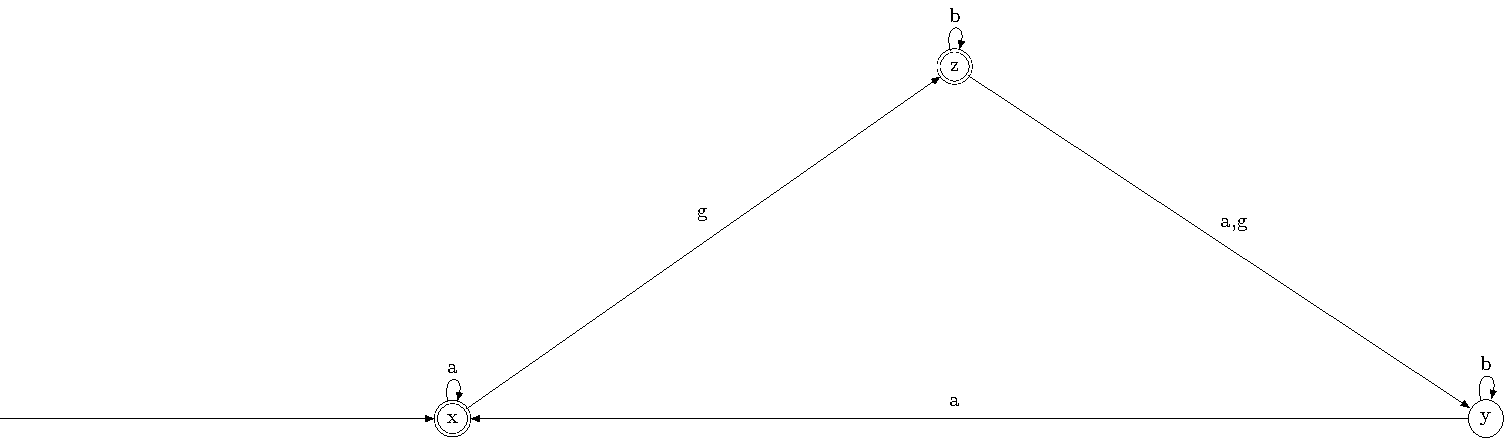
\includegraphics[width=1\textwidth]{automata/daoct/example.tikz}
  % \includetikzfigure[width=0.5\textwidth]{automata/example/example}
  \caption{Diagrama de transição de estados para $k=1$.}
  \label{fig:examplek1}
\end{figure}

\end{frame}

\begin{frame}{}
  \note{em geral aumentam o número de estados e diminuem os ciclos}
\begin{figure}[H]
    \footnotesize
  \centering 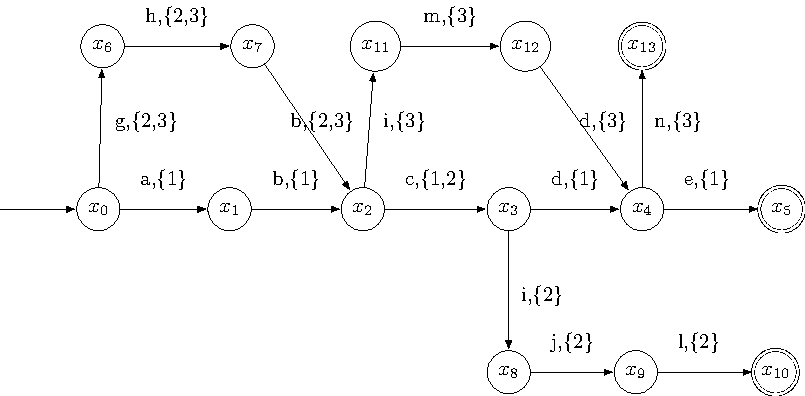
\includegraphics[width=0.9\textwidth]{automata/daoct/examplek2.tikz}
  % \includetikzfigure[width=0.5\textwidth]{automata/example/example}
  \caption{Diagrama de transição de estados para $k=2$.}
  \label{fig:examplek2}
\end{figure}
\end{frame}

%%% Local Variables:
%%% mode: latex
%%% TeX-master: "../presentation"
%%% End:

\tikzstyle{every picture}+=[remember picture]
\section{Projeto do Controlador a Eventos discretos}

\begin{frame}{Projeto do Controlador a Eventos discretos}
  \begin{enumerate}
   \item Projetar o controle\pause 
   \item Implementar o Controle \pause PLC - Ladder
\end{enumerate}
\end{frame}

\begin{frame}{Exemplo de Sistema}
\begin{figure}[H]
  \centering
  \includegraphics[width=0.8\textwidth]{cipnExample/schemePresentation.tikz}
  \caption{Exemplo de sistema a ser controlado.}
  \label{fig:cipnexamplescheme}
\end{figure}
% \note{
%   \begin{enumerate}
%    \item Projetar o controle\pause 
%    \item Implementar o Controle \pause PLC - Ladder \pause
%    \item Observar entradas e saídas\pause
%    \item Obter caminhos\pause
%    \item Identificar usando DAOCT 
%    \end{enumerate}
%  }
\end{frame}


\begin{frame}{Rede de Petri Interpretada para Controle}
\begin{figure}[H]
  \centering \includegraphics[width=\textwidth]{cipnExample/cipnPresentation.tikz}
  \caption{Exemplo de Rede de Petri interpretada para controle.}
  \label{fig:cipnexample}
\end{figure}
\end{frame}

\begin{frame}
  \begin{figure}[H]
    \centering
    \resizebox{0.7\textwidth}{!}{
   \includegraphics{cipnExample/cipnLadderPresentation.tikz}}
 \caption{Rede de Petri do exemplo implementada em Ladder.}
  \label{fig:cipnexampleLadder}
\end{figure}\note{método demonstrado por MOREIRA e BASILIO (2013)}
\end{frame}

\begin{frame}{Datalog}
  \note{
    Uma vez implementado o controle no PLC, é feita a observação. PLC Siemens possui
    os blocos functionais mostrados para gravar os dados num arquivo csv.\\
    Explicar cada bloco
  }
   \begin{figure}[ht]
       \begin{minipage}[b]{0.3\linewidth}
         \centering
 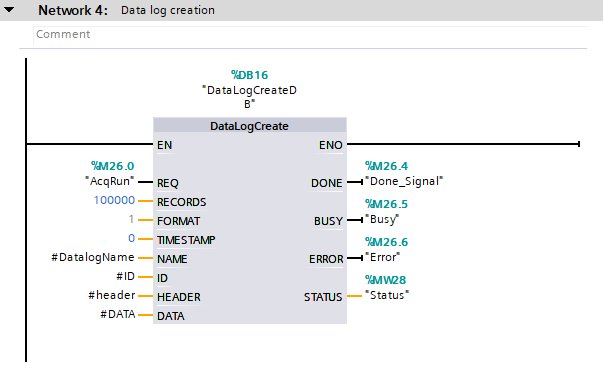
\includegraphics[width=\textwidth,clip,trim={0 0.8cm 3cm 0}]{tutorial/create}
       \end{minipage}
       \begin{minipage}[b]{0.3\linewidth}
         \centering
 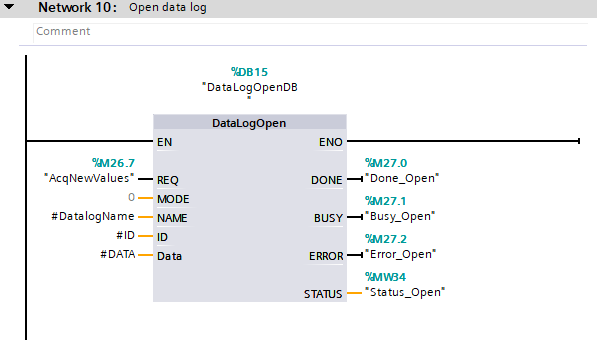
\includegraphics[width=\textwidth,clip,trim={0 0.4cm 3cm 0}]{tutorial/open}
\end{minipage}
       \begin{minipage}[b]{0.3\linewidth}
         \centering
	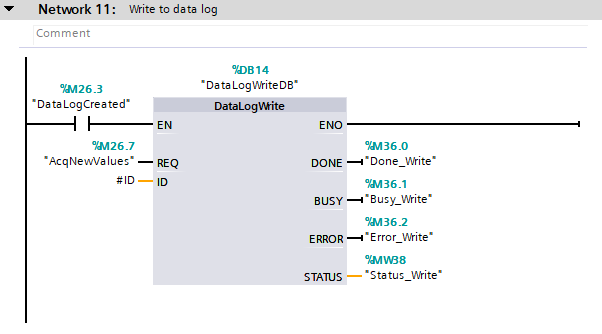
\includegraphics[width=\textwidth,clip,trim={0 0 3cm 0}]{tutorial/write}
       \end{minipage}
       \hspace{0.5cm}
       \begin{minipage}[b]{0.3\linewidth}
           \centering
	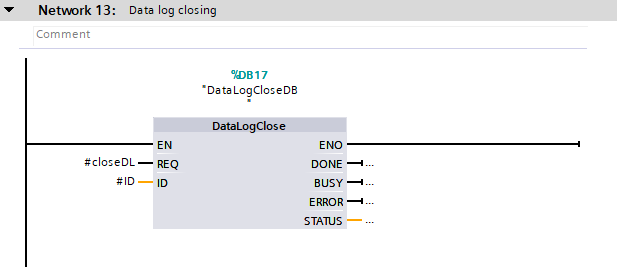
\includegraphics[width=\textwidth,clip,trim={0 1cm -3cm 0}]{tutorial/close}
       \end{minipage}
       \begin{minipage}[b]{0.3\linewidth}
           \centering
           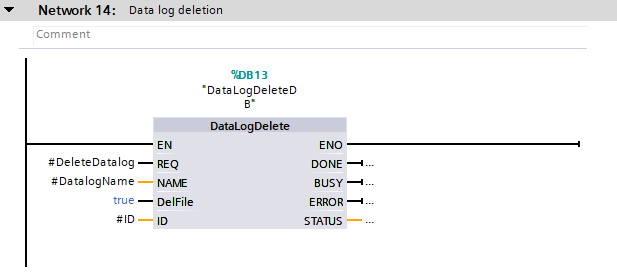
\includegraphics[width=\textwidth,clip,trim={0 -0.8cm 3cm 0}]{tutorial/delete}
       \end{minipage}
  \caption{Blocos Funcionais para gravação de dados.}
   \end{figure}
\end{frame}


\begin{frame} \begin{figure}
    \centering
\begin{tikzpicture}[scale=0.8]
     \def\corner{0.15in};
     \def\cornerradius{0.02in};
     \def\lwidth{0.02in};
     \def\h{1.1in};
     \def\w{0.85in};
     \def\nline{10};
     \def\iconmargin{0.1in};
     \def\topmargin{0.3in};
     \foreach[count=\i] \filename in {file.csv}
     {
     \coordinate (nw) at ($(-0.05in*\i,-0.15in*\i)$);
     \coordinate (ne0) at ($(nw) + (\w, 0)$);
     \coordinate (ne1) at ($(ne0) - (\corner, 0)$);
     \coordinate (ne2) at ($(ne0) - (0, \corner)$);
     \coordinate (se) at ($(ne0) + (0, -\h)$); 
     \filldraw [-, line width = \lwidth, fill=white] (nw) -- (ne1) -- (ne2)
      [rounded corners=\cornerradius]--(se) -- (nw|-se) -- cycle;
     \draw [-, line width = \lwidth] (ne1) [rounded corners=\cornerradius]-- (ne1|-ne2) -- (ne2);
     \node [anchor=north west] at (nw) {\scriptsize \tt \filename};
     \foreach \k in {1,...,\nline}
     {
       \draw [-, line width = \lwidth, line cap=round] 
         ($(nw|-se) + (\iconmargin,\iconmargin) + (0,{(\k-1)/(\nline-1)*(\h - \iconmargin - \topmargin)})$)
           -- ++ ($(\w,0) - 2*(\iconmargin,0)$);
     }
   }
   \node[inner sep=0pt] at (8,0) {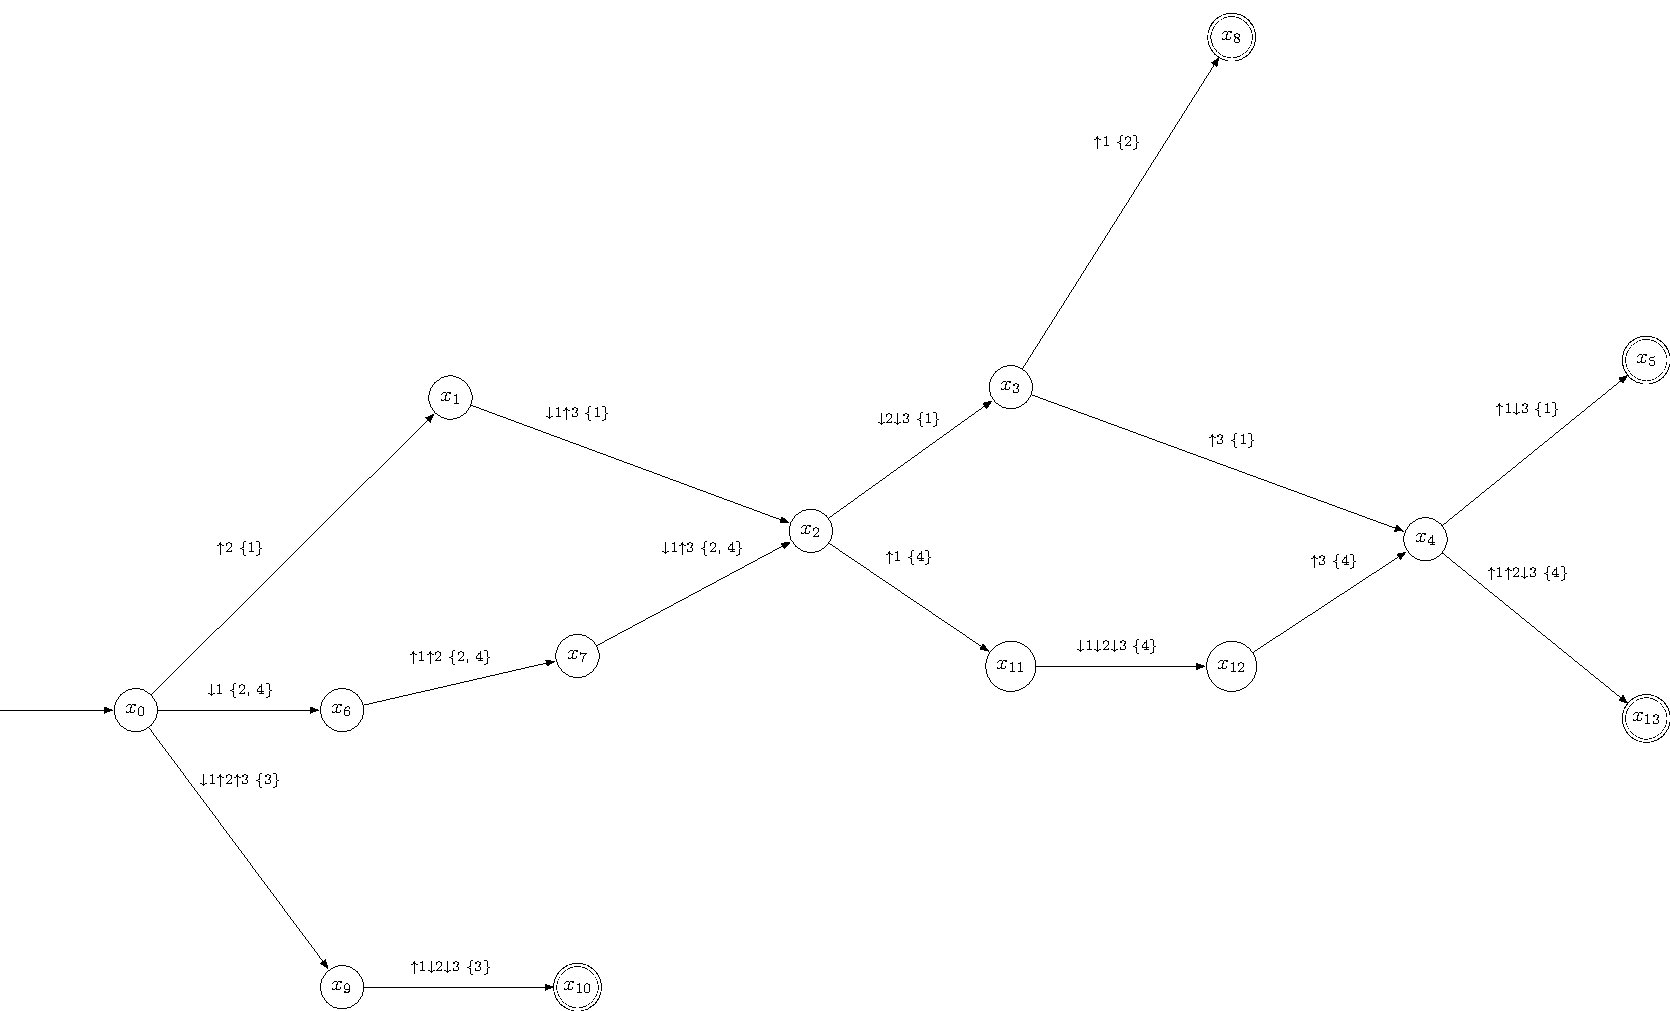
\includegraphics[width=0.4\textwidth]{example/example.pdf}};
   \draw[->] (1,0) to [bend left] (6,1);
   \draw (4,1.7) node {daoct};
   \end{tikzpicture}
  % \includetikzfigure[width=\textwidth]{example/stdin}
  \caption{Modelo identificado a partir do arquivo csv.}
  % \label{fig:identExamplekone}
\end{figure}
\note{
progama daoct criado para fazer obtenção dos caminhos da forma mostrada no
capítulo anterior, modificar os caminhos usando a formula descrita e
implementar o algoritmo de modelagemdo DAOCT.
}
\end{frame}

%%% Local Variables:
%%% mode: latex
%%% TeX-master: "../presentation"
%%% End:

\chapter{System}
\label{chap:system}
In this chapter, the system to be control and identified is presented.
The system is a didactic manufacture system assembled from submodules fabricated
by Christiani\footnote{All images from the Christiani modules are present on its sales
  catalog, available at \url{www.christiani.de}. All rights are reserved to Christiani.}, a German
constructor specialised in Mechatronic Systems and Industry Models to
didactic ends.
This manufacture system is located in the \LCA, situated in the \UFRJ. This
system is normally used for the under-graduated studies about Industrial
Automation and control of \DESs, and also for data acquisition in some
bachelor\slash master\slash doctorate thesis, as this one.

This manufacture system is a cube assembly system, where the different cube
halves shown in \autoref{fig:cubeHalves} are put together to form cubes.
\begin{figure}[H]
  \centering
  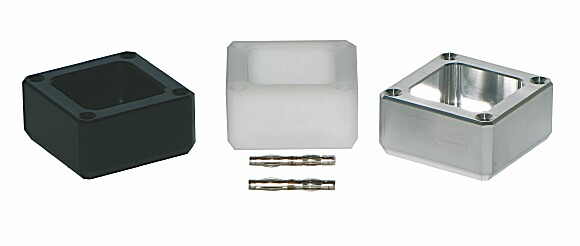
\includegraphics[width=0.55\textwidth]{maquete/pieces/workPieces.jpg}
  \caption{Cube halves.}
  \label{fig:cubeHalves}
\end{figure}

The pieces can be of two materials, metal or plastic, and the plastic ones can
be white or black.
The
permutation of cube halves needed to form a cube is selected via a type of
sorting, selecting the type of piece by material and colour. The assembled cubes
are then stored. In order to perform these tasks (sorting, handling, assembling
and stocking), 6 Units from Christiani manufacturer are used. These units can be
seen in \autoref{fig:units}.

\begin{figure}[H]
\begin{subfigure}[t]{0.35\textwidth}
  \centering
  \includegraphics[width=\textwidth]{maquete/mag/mag.jpg}
  \caption{Magazine Unit}
\end{subfigure}
\hfill
\begin{subfigure}[t]{0.35\textwidth}
  \centering
  \includegraphics[width=\textwidth]{maquete/esteira/esteira.jpg}
  \caption{Conveyor Belt.}
\end{subfigure}

\begin{subfigure}[t]{0.35\textwidth}
  \centering
  \includegraphics[width=\textwidth]{maquete/sensores/sensores.jpg}
  \caption{Sorting Unit.}
\end{subfigure}
\hfill
\begin{subfigure}[t]{0.35\textwidth}
  \centering
  \includegraphics[width=\textwidth]{maquete/braco/braco.jpg}
  \caption{Handling Unit.}
\end{subfigure}

\begin{subfigure}[t]{0.35\textwidth}
  \centering
  \includegraphics[width=\textwidth]{maquete/prensa/prensa.jpg}
  \caption{Assembly Unit.}
\end{subfigure}
\hfill
\begin{subfigure}[t]{0.35\textwidth}
  \centering
  \includegraphics[width=\textwidth]{maquete/elevador/elevador.jpg}
  \caption{Storage Unit.}
\end{subfigure}
  \caption{Units of the Manufacture System.}
  \label{fig:units}
\end{figure}

In the next sections each unit and their Inputs\slash Outputs will be detailed.

\begin{observation}
What is described in the next sections as an input of a certain module, it is
considered as an output for the controller and vice versa.  
\end{observation}

\section{Magazine Unit}
\label{sec:magazine}
The magazine is a unit with the objective to stock the cube halves to be used.
There are 2 types of magazines, one to stock pieces without connection pins (the pins shown in \autoref{fig:cubeHalves}) and another to
 stock pieces with those pins inserted, they can stack 10 and 8 pieces
 respectively. They will be denominated \verb| MAG 1| and \verb|MAG 2|.
Each magazine has a cylinder and a presence button. The cylinder serves to extract a
piece from the bottom of the stack, and the button to know if the stack is empty
or not. These cylinders have 2 inputs and 2
outputs. The inputs they are used to extend and retract the cylinders (if they
are set to $true$) and the
outputs are used to know if the cylinders are extended or retracted, the output
is equal to $true$ if the respective condition is fulfilled. These
inputs  are called in this work \verb|Extend MAG 1/2 Cylinder| and
\verb|Retract MAG 1/2 Cylinder|, and the outputs are called \verb|MAG 1/2 Cylinder Extended| and
\verb|MAG 1/2 Cylinder Retracted|. The presence button of each magazine outputs a $true$
value if the stack is empty and $false$, otherwise. Thus this presence buttons
are called in this work \verb|MAG 1/2 Empty|, their localisation on the magazine
can be seen in \autoref{fig:magazine2}. 
\begin{figure}[H]
  \centering
  \begin{tikzpicture}
    \node[anchor=south west,inner sep=0] (image) at (0,0) {
      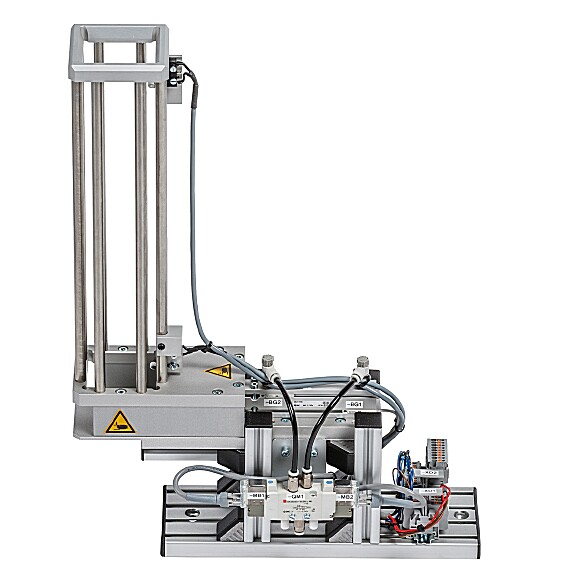
\includegraphics[width=8cm]{maquete/mag/30540_4.jpg}
    };
    % \draw[red,ultra thick,rounded corners] (0,0) rectangle (9.4,6.2);
    \begin{scope}[x={(image.south east)},y={(image.north west)}]
        % \draw[help lines,xstep=.1,ystep=.1] (0,0) grid (1,1);
        % \foreach \x in {0,1,...,9} { \node [anchor=north] at (\x/10,0) {0.\x}; }
        % \foreach \y in {0,1,...,9} { \node [anchor=east] at (0,\y/10) {0.\y}; }
      \draw[red] (0.85,0.55) node {\textbf{Cylinder}};
      \draw[<-,>=stealth,red,very thick] (0.8,0.5) -- (0.67,0.37);
      \draw[red] (0.75,0.7) node {\textbf{Presence Button}};
      \draw[red,very thick, rounded corners] (0.25,0.35) rectangle (0.35,0.45);
      \draw[<-,>=stealth,red,very thick] (0.6,0.65) -- (0.37,0.45);
      \end{scope}
  \end{tikzpicture}
  \caption{Magazine Unit}
  \label{fig:magazine2}
\end{figure}

% only presence button
% \begin{figure}[H]
%   \centering
%   \begin{tikzpicture}
%     \node[anchor=south west,inner sep=0] (image) at (0,0) {
%       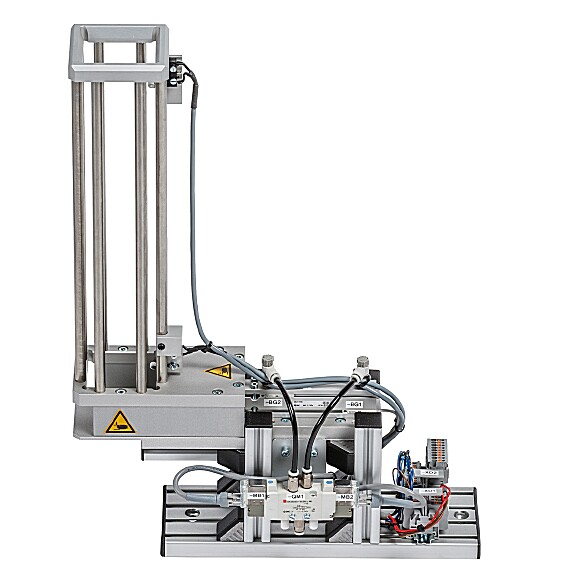
\includegraphics[width=8cm]{maquete/mag/30540_4.jpg}
%     };
%     % \draw[red,ultra thick,rounded corners] (0,0) rectangle (9.4,6.2);
%     \begin{scope}[x={(image.south east)},y={(image.north west)}]
%         % \draw[help lines,xstep=.1,ystep=.1] (0,0) grid (1,1);
%         % \foreach \x in {0,1,...,9} { \node [anchor=north] at (\x/10,0) {0.\x}; }
%         % \foreach \y in {0,1,...,9} { \node [anchor=east] at (0,\y/10) {0.\y}; }
%       \draw[red] (0.75,0.5) node {\textbf{Presence Button}};
%       \draw[red,very thick, rounded corners] (0.25,0.35) rectangle (0.35,0.45);
%       \draw[->,red,very thick] (0.5,0.5) -- (0.37,0.45);
%       \end{scope}
%   \end{tikzpicture}
%   \caption{Magazine Unit}
% \end{figure}

\section{Conveyor Belt}
\label{sec:magazine}
The conveyor belt is a unit with the objective of transporting the pieces from a
unit to another. It has 2 inputs and 1 output. The inputs are used to turn the
belt on, but each input makes it turn in a direction or the other. The output is
the generated by a presence sensor located in on extremity of the belt (see
\Autoref{fig:conveyorBelt}), it is equal to $true$ if there is a piece in front
of it and $false$ otherwise. The directions of the movement of the pieces is
denominated Forward if it is going towards the presence sensor and reverse if
not. Thus the names given to the inputs that generate this movements are
\verb|Conveyor Belt Forward| and \verb|Conveyor Belt Reverse|.
And the input is called \verb|Proximity Sensor End of Conveyor Belt|.

\begin{figure}[H]
  \centering
  \begin{tikzpicture}
    \node[anchor=south west,inner sep=0] (image) at (0,0) {
      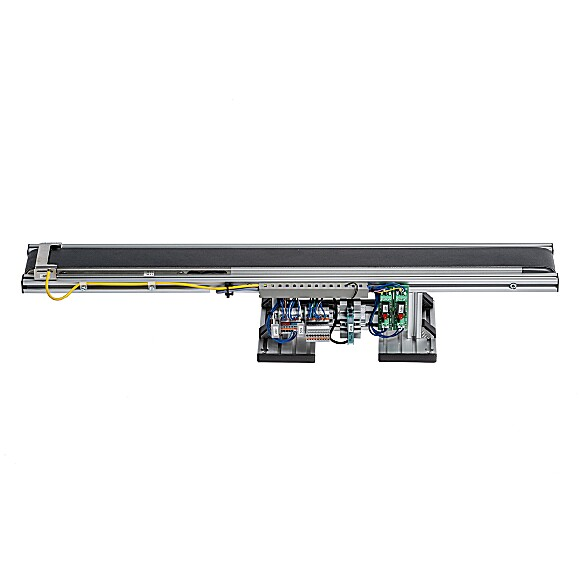
\includegraphics[trim={0 6cm 0 5cm},clip,width=8cm]{maquete/esteira/40778_3.jpg}
    };
    % \draw[red,ultra thick,rounded corners] (0,0) rectangle (9.4,6.2);
    \begin{scope}[x={(image.south east)},y={(image.north west)}]
        % \draw[help lines,xstep=.1,ystep=.1] (0,0) grid (1,1);
        % \foreach \x in {0,1,...,9} { \node [anchor=north] at (\x/10,0) {0.\x}; }
        % \foreach \y in {0,1,...,9} { \node [anchor=east] at (0,\y/10) {0.\y}; }
        \draw [->,>=stealth,red, very thick](0.9,0.75) -- ++ (-0.8,0.0);
        \draw [red] (0.5,0.85) node {Forward};
        \draw [->,>=stealth,red, very thick](0.1,0.95) -- ++ (0.8,0.0);
        \draw [red](0.5,1.05) node {Reverse};
        
        \draw [red](0.5,0.0) node {Presence Sensor};
        \draw [red,very thick,rounded corners](0.05,0.45) rectangle (0.12,0.65);
        \draw [->,>=stealth,red, very thick](0.1,0.4) -- (0.3,0.1);
      \end{scope}
  \end{tikzpicture}
  \caption{Conveyor Belt}
  \label{fig:conveyorBelt}
\end{figure}

% no sensor
% \begin{figure}[H]
%   \centering
%   \begin{tikzpicture}
%     \node[anchor=south west,inner sep=0] (image) at (0,0) {
%       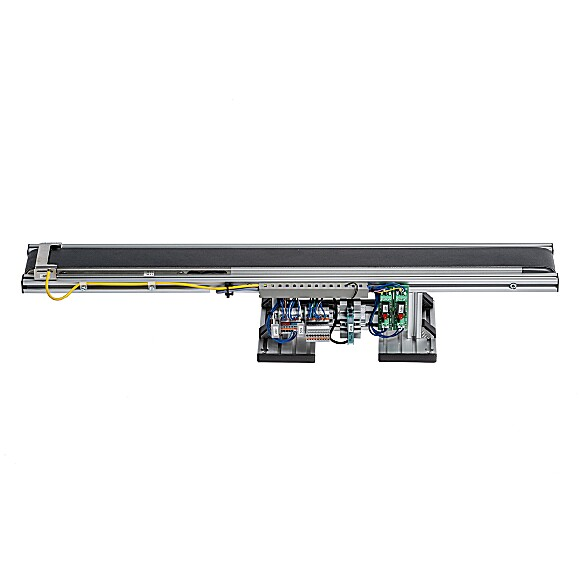
\includegraphics[trim={0 6cm 0 5cm},clip,width=8cm]{maquete/esteira/40778_3.jpg}
%     };
%     % \draw[red,ultra thick,rounded corners] (0,0) rectangle (9.4,6.2);
%     \begin{scope}[x={(image.south east)},y={(image.north west)}]
%         % \draw[help lines,xstep=.1,ystep=.1] (0,0) grid (1,1);
%         % \foreach \x in {0,1,...,9} { \node [anchor=north] at (\x/10,0) {0.\x}; }
%         % \foreach \y in {0,1,...,9} { \node [anchor=east] at (0,\y/10) {0.\y}; }
%         \draw [->,>=stealth,red, very thick](0.9,0.7) -- (0.1,0.7);
%         \draw [red] (0.5,0.8) node {Forward};
%         \draw [->,>=stealth,red, very thick](0.1,0.1) -- (0.9,0.1);
%         \draw [red](0.5,0.0) node {Reverse};
%       \end{scope}
%   \end{tikzpicture}
%   \caption{Conveyor Belt}
% \end{figure}

\section{Sorting Unit}
\label{sec:sortingUnit}
As the name says, the sorting unit serves to sort the pieces. 
\begin{figure}[H]
  \centering
  \begin{tikzpicture}
    \node[anchor=south west,inner sep=0] (image) at (0,0) {
      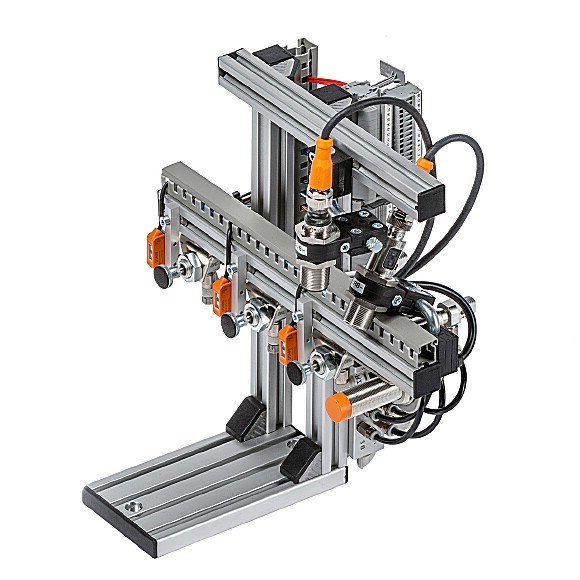
\includegraphics[trim={0 0 0 0},clip,width=8cm]{maquete/sensores/69511_2.jpg}
    };
    % \draw[red,ultra thick,rounded corners] (0,0) rectangle (9.4,6.2);

    \begin{scope}[x={(image.south east)},y={(image.north west)}]
        \draw[help lines,xstep=.1,ystep=.1] (0,0) grid (1,1);
        \foreach \x in {0,1,...,9} { \node [anchor=north] at (\x/10,0) {0.\x}; }
        \foreach \y in {0,1,...,9} { \node [anchor=east] at (0,\y/10) {0.\y};  }
        \draw[red,ultra thick,rounded corners] (0.15,0.4) rectangle ++ (0.15,0.1);
        \draw[red] (0.1,0.1) node {\textbf{Left}};
        \draw[->,>=stealth,red, very thick] (0.2,0.38) -- (0.1,0.15);
        \draw[magenta,ultra thick,rounded corners] (0.35,0.4) rectangle ++ (0.15,0.1);
        \draw[magenta] (0.1,0.8) node {\textbf{Center}};
        \draw[->,>=stealth,magenta, very thick] (0.4,0.52) -- (0.2,0.75);
        \draw[cyan,ultra thick,rounded corners] (0.53,0.4) rectangle ++ (0.15,0.1);
        \draw[cyan] (0.7,0.1) node {\textbf{Right}};
        \draw[->,>=stealth,cyan, very thick] (0.65,0.38) -- (0.7,0.15);
      \end{scope}
  \end{tikzpicture}
  \caption{Sorting Unit - Identification}
  \label{fig:sortIden}
\end{figure}
\begin{figure}[H]
  \centering
  \begin{tikzpicture}
    \node[anchor=south west,inner sep=0] (image) at (0,0) {
      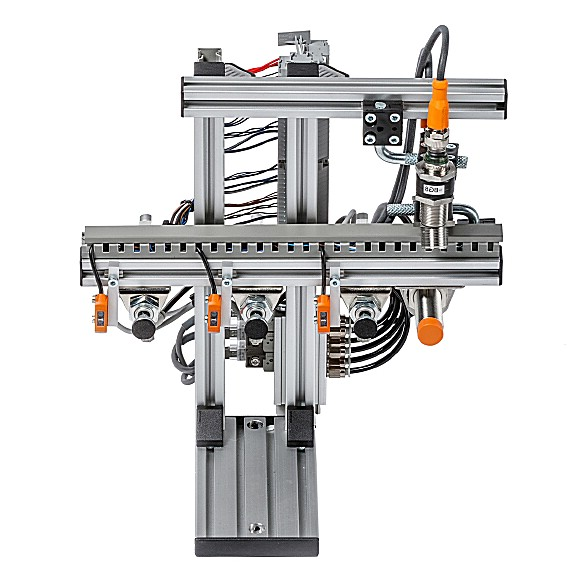
\includegraphics[trim={0 0 0 0},clip,width=8cm]{maquete/sensores/69511_3.jpg}
    };
    % \draw[red,ultra thick,rounded corners] (0,0) rectangle (9.4,6.2);

    \begin{scope}[x={(image.south east)},y={(image.north west)}]
        % \draw[help lines,xstep=.1,ystep=.1] (0,0) grid (1,1);
        % \foreach \x in {0,1,...,9} { \node [anchor=north] at (\x/10,0) {0.\x}; }
        % \foreach \y in {0,1,...,9} { \node [anchor=east] at (0,\y/10) {0.\y};  }
        \draw[red,ultra thick,rounded corners] (0.15,0.4) rectangle ++ (0.15,0.1);
        \draw[red] (0.1,0.1) node {\textbf{Left}};
        \draw[->,>=stealth,red, very thick] (0.2,0.38) -- (0.1,0.15);
        \draw[magenta,ultra thick,rounded corners] (0.35,0.4) rectangle ++ (0.15,0.1);
        \draw[magenta] (0.1,0.8) node {\textbf{Center}};
        \draw[->,>=stealth,magenta, very thick] (0.4,0.52) -- (0.2,0.75);
        \draw[cyan,ultra thick,rounded corners] (0.53,0.4) rectangle ++ (0.15,0.1);
        \draw[cyan] (0.7,0.1) node {\textbf{Right}};
        \draw[->,>=stealth,cyan, very thick] (0.65,0.38) -- (0.7,0.15);
      \end{scope}
  \end{tikzpicture}
  \caption{Sorting Unit - Discharge}
  \label{fig:sortDisc}
\end{figure}

\section{Handling Unit}
\label{sec:handlingUnit}

\section{Assembly Unit}
\label{sec:assemblyUnit}

\section{Storage Unit}
\label{sec:storageUnit}
\begin{figure}[H]
  \centering
  \begin{tikzpicture}
    \node[anchor=south west,inner sep=0] (image) at (0,0) {
      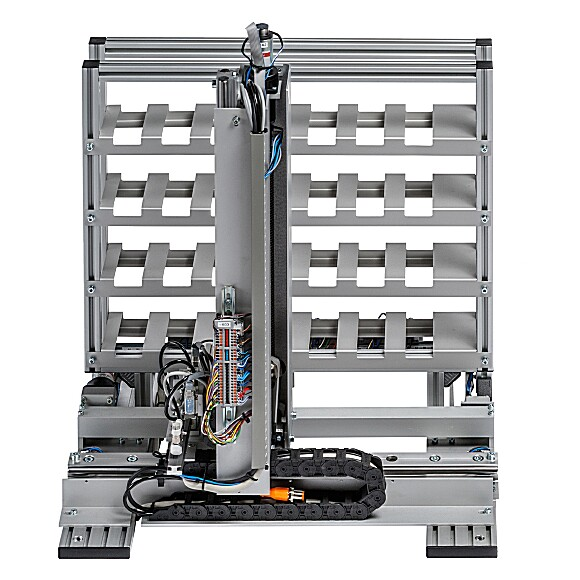
\includegraphics[width=8cm]{maquete/elevador/69523_3.jpg}
    };
    % \draw[red,ultra thick,rounded corners] (0,0) rectangle (9.4,6.2);
    \begin{scope}[x={(image.south east)},y={(image.north west)}]
        % \draw[help lines,xstep=.1,ystep=.1] (0,0) grid (1,1);
        % \foreach \x in {0,1,...,9} { \node [anchor=north] at (\x/10,0) {0.\x}; }
        % \foreach \y in {0,1,...,9} { \node [anchor=east] at (0,\y/10) {0.\y}; }
      \draw[red] (1,0.5) node {\textbf{Right}};
      \draw[red] (0,0.5) node {\textbf{Left}};
      \draw[red] (0.5,1) node {\textbf{Top}};
      \draw[red] (0.5,0) node {\textbf{Bottom}};
      \end{scope}
  \end{tikzpicture}
  \caption{Storage Unit}
\end{figure}


%%% Local Variables:
%%% mode: latex
%%% TeX-master: "../monografia"
%%% End:

\chapter{Results}
\label{cha:results}

In this 2 paths
best 80 paths States
all
1321  2166  2962  3744  4508  5235  5939

best
1294  2127  2904  3663  4395  5088  5746
\begin{figure}[H]
  \centering
  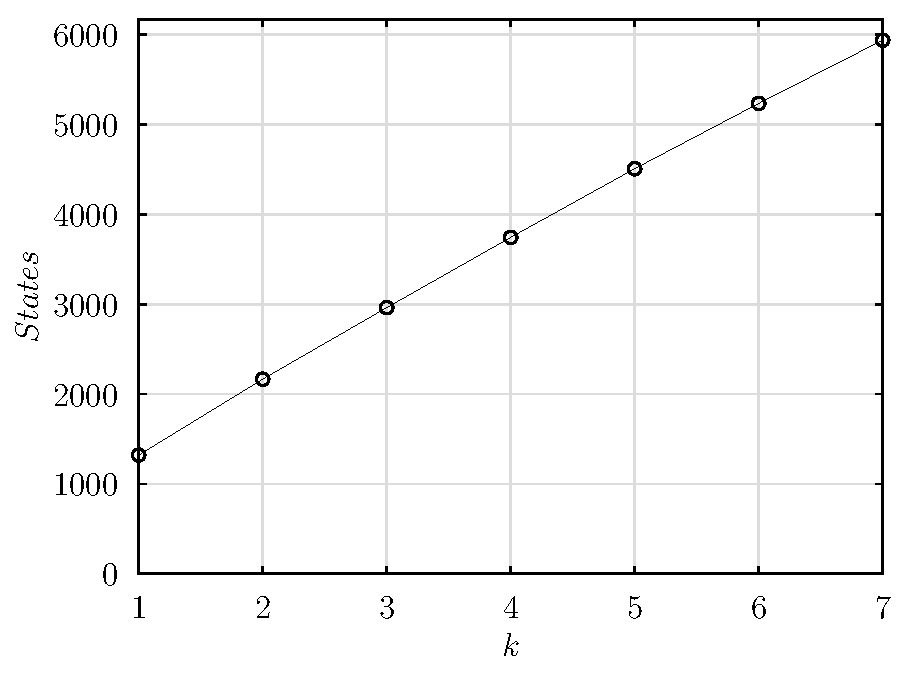
\includegraphics[width=0.5\textwidth]{results/all/states.pdf}
  \caption{Input\slash Output Process model}
    \label{fig:ioProcModel}
\end{figure}
\begin{figure}[H]
  \centering
  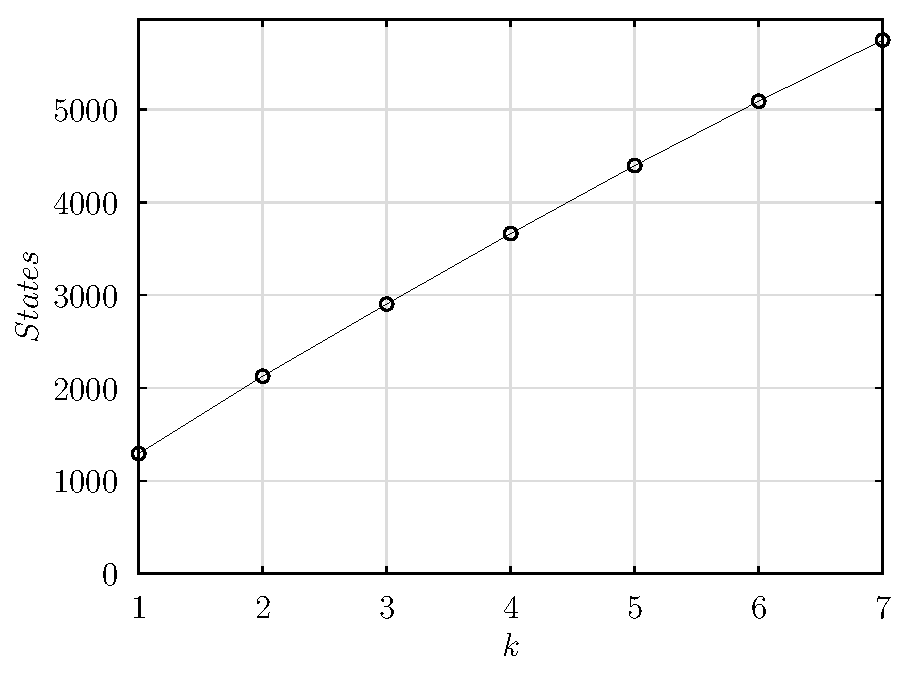
\includegraphics[width=0.5\textwidth]{results/all/best/states.pdf}
  \caption{Input\slash Output Process model}
    \label{fig:ioProcModel}
\end{figure}
\begin{figure}[H]
  \centering
  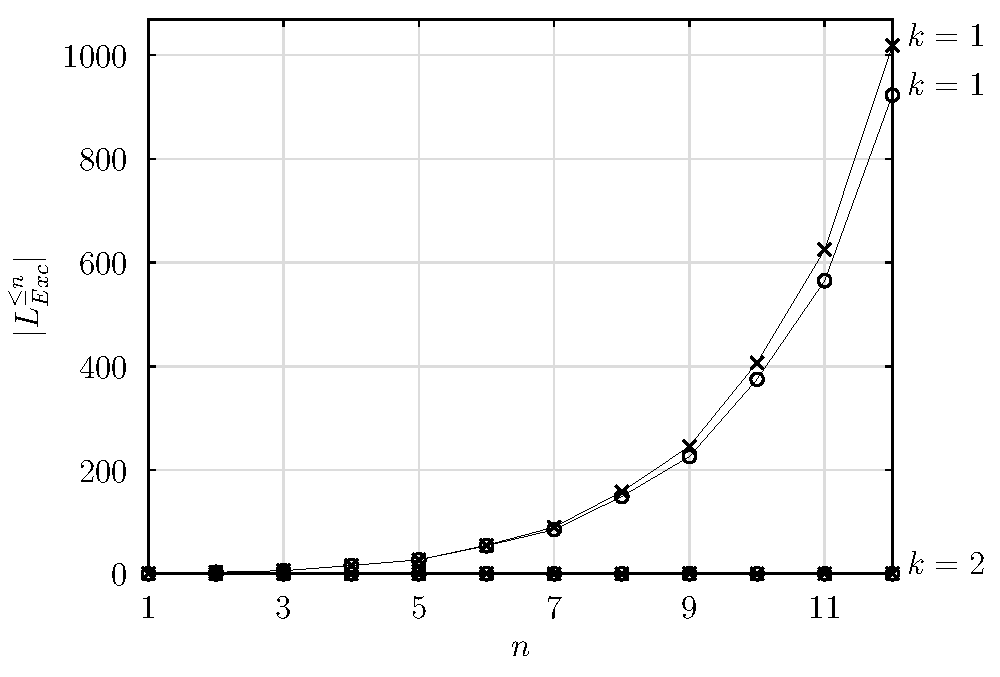
\includegraphics[width=0.5\textwidth]{results/all/exceedingLanguage-daoct-ndaao_k1-2_n12.pdf}
  \caption{Input\slash Output Process model}
    \label{fig:ioProcModel}
\end{figure}

 \section{best} 
\begin{figure}[H]
\begin{subfigure}[H]{0.5\textwidth}
  \centering
  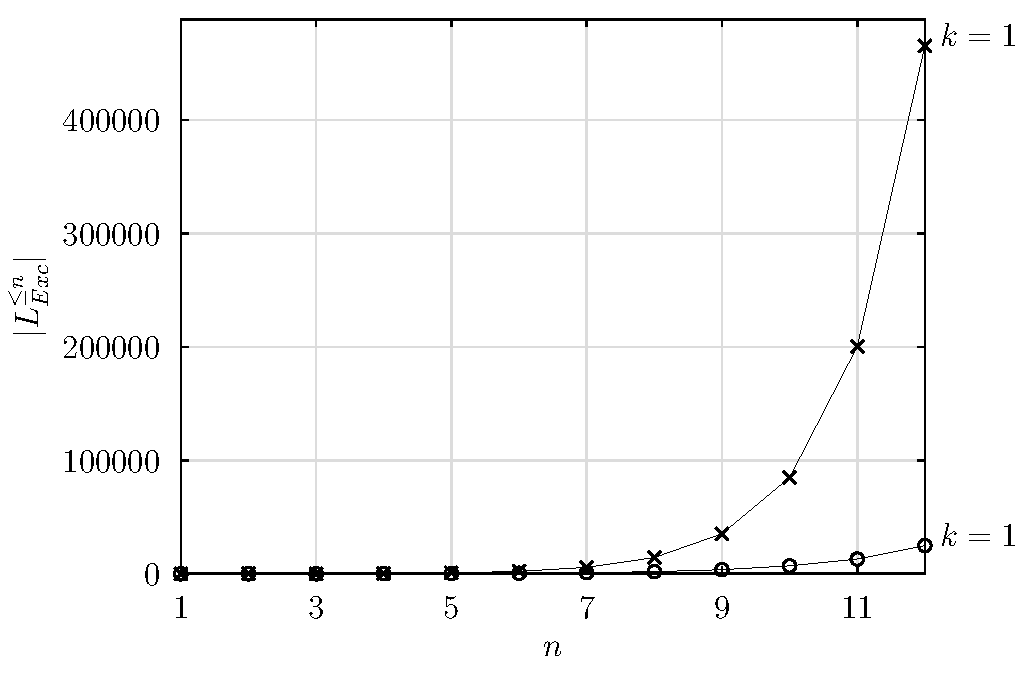
\includegraphics[width=\textwidth]{results/all/best/exceedingLanguage-daoct-ndaao_k1_n12.pdf}
  \caption{Input\slash Output Process model}
    \label{fig:ioProcModel}
\end{subfigure}
\begin{subfigure}[h]{0.5\textwidth}
  \centering
  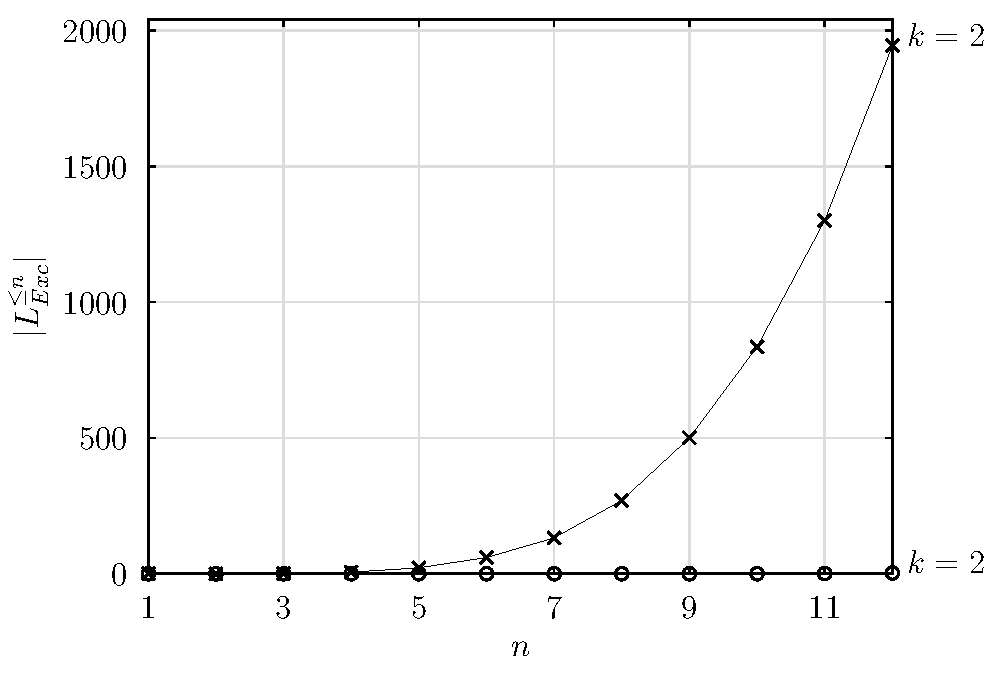
\includegraphics[width=\textwidth]{results/all/best/exceedingLanguage-daoct-ndaao_k2_n12.pdf}
  \caption{Input\slash Output Process model}
    \label{fig:ioProcModel}
\end{subfigure}
\end{figure}
\section{DAOCT}
\label{sec:results_daoct}

\section{Discussion about the identification}
\begin{figure}[H]
  \centering
  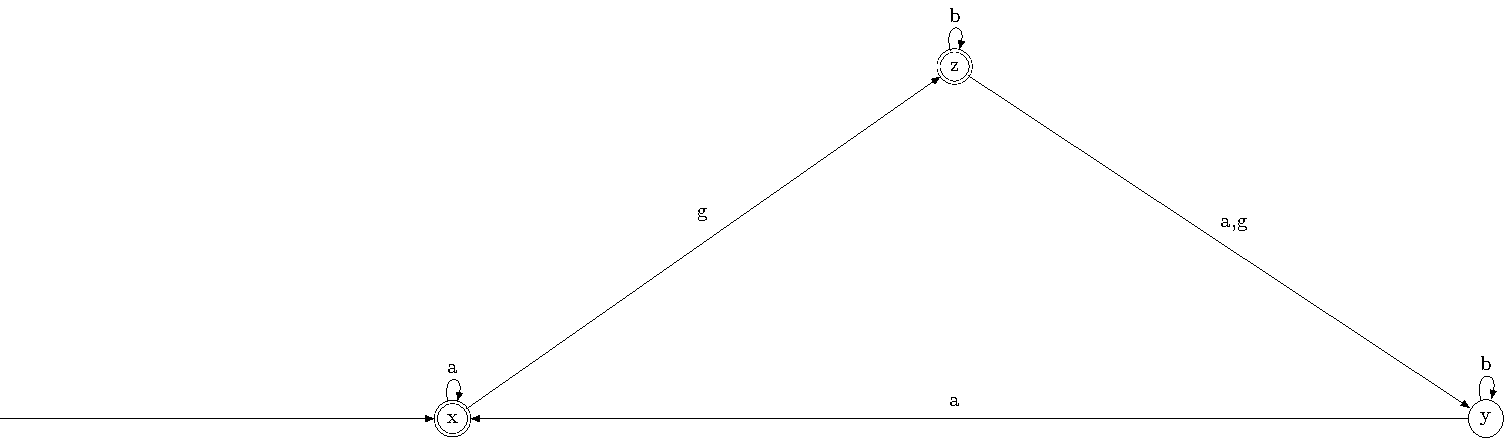
\includegraphics{results/example/example}
  \caption{Input\slash Output Process model}
    \label{fig:ioProcModel}
\end{figure}


\begin{figure}[H]
  \centering
  \includegraphics{results/example/examplek1NoArrows}
  \caption{Input\slash Output Process model}
    \label{fig:ioProcModel}
\end{figure}

\begin{figure}[H]
  \centering
  \includegraphics{results/example/example1k1NoArrows}
  \caption{Input\slash Output Process model}
    \label{fig:ioProcModel}
\end{figure}

\begin{figure}[H]
  \centering
  \includegraphics{results/example/example1k2NoArrows}
  \caption{Input\slash Output Process model}
    \label{fig:ioProcModel}
\end{figure}
% \begin{figure}[H]
%   \centering
%   \includegraphics[width=0.5\textwidth]{exceedingLanguage/example/exceedingLanguage-daoct-ndaao_k2_n7.pdf}
%   \caption{Cardinality of the exceeding language of the DAOCT (o) and NDAAO
%     ($\times$) models. $k = 1$, and $1 \leq n \leq 7$}
%   \label{fig:exceedingLangExample}
% \end{figure}


% Comparing the results of the \autoref{fig:exceedingLangExample}  with the
% example 3 from \cite{moreira2018enhanced}, we can
% observe that the exceeding language for the DAOCT model drops. This is caused by
% how the acquisition works, in this work, the plant is considered a black box, so
% instead of feeding the algorithm with the
% paths, the raw data is given, and the paths are calculated using the first
% IO\_Vector as the initial state and once this initial state is repeated other
% path 
% is created, resulting on 4 paths instead of 3. This change, can result in a
% smaller path, with no loops, diminishing the exceeding language.


% \section{Manufacture System}
% \label{sec:results_system}

% \begin{figure}[H]
%   \centering
%   \includegraphics[width=0.5\textwidth]{results/all/exceedingLanguage-daoct-ndaao_k1_n7.pdf}
%   \caption{graph}
% \end{figure}

% \begin{figure}[H]
%   \centering
%   \includegraphics[width=0.5\textwidth]{results/all/exceedingLanguage-daoct-ndaao_k2-3-7_n25.pdf}
%   \caption{graph}
% \end{figure}

% \todo{Choosing the IO\_Vector with the greatest repetition ratio as $x_0$}

% \begin{figure}[H]
%   \centering
%   \includegraphics[width=0.5\textwidth]{results/all/best/exceedingLanguage-daoct-ndaao_k1_n7.pdf}
%   \caption{graph}
% \end{figure}


% \begin{figure}[H]
%   \centering
%   \includegraphics[width=0.5\textwidth]{results/all/best/exceedingLanguage-daoct-ndaao_k2-3-7_n25.pdf}
%   \caption{graph}
% \end{figure}

% Removing I\_MAG1EMPT and I\_MAG2EMPT

% \begin{figure}[H]
%   \centering
%   \includegraphics[width=0.5\textwidth]{results/all-2_5/exceedingLanguage-daoct-ndaao_k1_n7.pdf}
%   \caption{graph}
% \end{figure}

% \todo{Choosing the IO\_Vector with the greatest repetition ratio as $x_0$}

% \begin{figure}[H]
%   \centering
%   \includegraphics[width=0.5\textwidth]{results/all-2_5/best/exceedingLanguage-daoct-ndaao_k1_n7.pdf}
%   \caption{graph}
% \end{figure}

% As we can see, the exceedingLanguage raises




%%% Local Variables:
%%% mode: latex
%%% TeX-master: "../monografia"
%%% End:

\chapter{Conclusion}
\label{cha:conclusion}
% As proposed in the introduction, this work presents a methodology and tools for
% control, observation and identification of \DESs{} in order to have a model to be
% used for fault detection. In this chapter a brief retrospective of the process
% of preparation of the methodology and the tools presented is made. And then the
% conclusions are drawn based on the results generated by the application of
% the methodology
% to identify a didactic manufacturing system.
% The control implementation was based on the
% method shown in \cite{moreira2013bridging} and the identification model based on \cite{moreira2018enhanced}.
% This identification method based on the
% observation of the fault-free behaviour of the system
% acquisition , from its conception.

% Through the process of preparation of the methodology and tools, some issues
% were found, and they are compiled in this chapter. Some
% workarounds are proposed as new approaches to solve these issues in future works.

\section{Concluding Remarks}
\label{sec:concludingRemarks}
In this work a method for the control, observation and identification of a
\DES{} was presented. First, the control logic was created using a \CIPN, and then implemented
in \LD{} to be used in a Siemens \PLC{} (\Autoref{cha:control}). After that, the observation of the
inputs and outputs of the controller was made using data log function blocks that saved the data in
\verb|.csv| files, and finally, these \verb|.csv| files were used as the input of the
identification algorithm generating a \DAOCT{} model (\Autoref{cha:ident}). In
\Autoref{cha:results} we could see that if the system was observed for a long
time and the initial state of observation was well-chosen, then the \DAOCT{} is
a good candidate for modelling, if the aim of this modelling is fault-detection.
The fact that the exceeding language of the \DAOCT{} model drops to $0$ more
rapidly than other models, with a smaller value of the variable $k$, proves that it is less resource intensive than the
others, even for relatively big
systems, with more than $60$ inputs\slash outputs with concurrent behaviour.


\section{Further Work}
An issue found in the implementation of the control is the use of \LD{} to
program the logic. Although \LD{} is very used
in the industry, as it is a visual language, it creates a difficulty for the
automation of the conversion from Petri net. An approach that can be used in
future works would be to represent the Petri net in a text format, Petri net
markup language for instance (presented in \cite{weber2003petri}), and create a
tool that automatically converts this file to a text based language standardised
by the IEC 61131-1, \IL{} or \ST{}. Since \IL{} is less used, \ST{}
would be a better choice. Using a text based language increases portability
of the code and it helps the development, since version control can be used in
text files, allowing the collaboration of multiple people to edit the code if
needed, and track who made the changes, increasing the maintainability
of the code.



Another issue was about the observation. Although the acquisition of
inputs\slash outputs using data logs and saving the data in batches on
\verb|.csv| files can be used for the identification process, for
fault-detection it is not optimal to use this approach, a better one would be to
acquire the data in real time, by using some API, snap7 for example, or using
\SCADA{} protocols.
% But if we use in a future work the function block created to log
% the data in \Autoref{cha:ident}, the \emph{LOGDATA} block, it is recommended to
% optimise its contents. Some refactoring on the logic could be made, increasing its
% speed and removing some unnecessary variables that may be present.

As shown in \Autoref{cha:results}, the didactic manufacturing system used for the
experiments have a considerable concurrent behaviour, affecting the identified
model, on the number of states and extracted paths. As future work would be to divide the observation of the system in its modules, and
compare the multiple models generated by the identification algorithm with the
one using the observation of the complete system.

Another issue shown in \Autoref{cha:results}, is the choice of the first
vector to be used as initial state in the identification algorithm. Here we
propose for future works a study on how to find the optimal vector. Two
scenarios could be considered: the first one taking a grey box approach, where some behaviour
is previously known, by a simple description of the function of the system and another considering a black box approach.

Another proposition for a future work is made in \Autoref{cha:results}. Instead
of using an identification model based on the observation of inputs\slash
outputs of the system, an alternative would be to create and use a model that uses the observation of
the events of the system.


% to extract the paths and events of the system and to identify the system
% behaviour,
% a way out would be to observe the events and use them to identify the
% system. Of course the \DAOCT{} model would not be fit for it, and another model
% should be developed. This way, probably the problem with the choice of the
% initial state of the system would cease to exist.


%%% Local Variables:
%%% mode: latex
%%% TeX-master: "../monografia"
%%% End:


\appendix
\begin{frame}[allowframebreaks] %allow to expand references to multiple frames (slides)

\frametitle{References}

\scriptsize{\bibliographystyle{plainnat}}

\nocite{moreira2013bridging}
\bibliography{bibliography}
\end{frame}



\end{document}


% Examples
% convert video to theora
% ffmpeg2theora -i time-lapse.mp4  --videoquality 4 --optimize -o timelapse.avi
% \begin{frame}{Imagem}
% \begin{figure}
% \includegraphics[height=4cm]{../../videos/TCCVIDEO_HTML-HTMI.jpg}
% \caption{Figura}
% \end{figure}
% \end{frame}
% \begin{frame}{Video}
% \centering
% \href{run:../../videos/TCCVIDEO_HTML-HTMI.avi}{\includegraphics[width=0.7\textwidth]{../../videos/TCCVIDEO_HTML-HTMI.jpg}}
%  % \inlineMovie[]{../../videos/TCCVIDEO_HTML-HTMI.avi}{../../videos/TCCVIDEO_HTML-HTMI.jpg}{width=0.7\textwidth}
% \end{frame}

% \begin{frame}{Exemplo de frases espaçadas tipo Afonso}
% 	\onslide<1,2,3,5>{\quad First Line of Text}
% 	\only<2,3>{\\ \quad \quad Second Line of Text}
% 	\onslide<3>{\\ \quad \quad \quad Third Line of Text}
% \end{frame}
%\begin{frame}{Exemplo de frases espaçadas tipo Afonso}
%	\onslide<1,2,3,5>{\quad First Line of Text}
%	\only<2,3>{\\ \quad \quad Second Line of Text}
%	\onslide<3>{\\ \quad \quad \quad Third Line of Text}
%\end{frame}


%\begin{frame}
%\begin{enumerate}
%\item Item 1
%\end{enumerate}
%\begin{itemize}
%\item[\XSolidBrush] Item 1
%\end{itemize}
%\end{frame}
%
%\begin{frame}{Imagem}
%\begin{figure}
%\includegraphics[height=4cm]{redesbr.JPG}
%\caption{Figura}
%\end{figure}
%
%\end{frame}
%
%\begin{frame}{2 images same title}
%\begin{figure}
%   \includegraphics[width=0.475\textwidth]{redesbr.JPG}
%   \hfill
%   \includegraphics[width=0.475\textwidth]{redesbr.JPG}
%   \caption{Imagem tal esquerda e outra direita}
%\end{figure}
%\end{frame}
%
%\begin{frame}{2 images different titles}
%    \begin{figure}[ht]
%        \begin{minipage}[b]{0.45\linewidth}
%            \centering
%            \includegraphics[width=\textwidth]{redesbr}
%            \caption{Label for a}
%            \label{fig:a}
%        \end{minipage}
%        \hspace{0.5cm}
%        \begin{minipage}[b]{0.45\linewidth}
%            \centering
%            \includegraphics[width=\textwidth]{redesbr}
%            \caption{Label for b}
%            \label{fig:b}
%        \end{minipage}
%    \end{figure}
%\end{frame}
%}


